\section{Hardness Results}
\label{sec:hardness}


In this section we give hardness results for non-linear paging. In particular, we give a lower bound for supermodular paging based on a reduction from online set cover. This yields the proofs of \Cref{lem:Set Cover,thm:LB,thm:hardness}. We remark that the proof can be strengthened by providing a reduction from online submodular cover, however, we omit the details as we are not aware of stronger lower bounds for online submodular cover (compared to online set cover). In addition, in \Cref{sec:hardRestricted} we give a lower bound for solving non-linear paging in restricted cases. %online set cover and online submodular cover admit similar lower bounds \cite{alon2003online,korman2004use}.

 Recall that in online set cover we are given  a ground set $X = \{1,2,\ldots, n\} = [n]$ and a family $\cS = \{S_1,\ldots, S_m\}$ of subsets of $X$ (note that in this section only $n$ does not describes the number of pages). Requests for certain elements from $X$ arrive online; let $i_t$ be the requested element in time $t$ for a set of time steps $T$. If the requested element is not covered by a previously chosen set, we choose a set $S \in \cS$ containing the element to cover it, paying a cost $c(S)$. The goal is to minimize the cost of selected sets. Throughout this section, we fix the arbitrary online set cover instance $I$ described above. 

We construct a reduced supermodular paging instance $R_I$. Define the set of pages as $\cP = X \cup \cS$; that is, we define a page for every element and every set of the online set cover instance $I$. Define a cost $c(i) = \infty$ for every element $i \in [n]$ and for every set $S \in \cS$ we keep the original cost $c(S)$ from the set cover instance $I$ also as the cost for the supermodular paging instance $R_I$. Finally, define the cover function $g: 2^{\cP} \rightarrow \mathbb{N}$ such that for all $F \subseteq \cP$ 
\begin{equation}
	\label{eq:g}
	g(F) = \left| \{i \in X~|~ \exists S \in \cS \cap F \text{ s.t. } i \in S\} \cup \left(X \cap F\right) \right|. 
\end{equation} In simple words, $g(F)$ describes the number of elements $i$ in $X$ {\em covered} either by a set $S$ (i.e., $i \in S$) that belongs to $F$ or by the actual corresponding element that belongs to $F$ (i.e., $i \in F$). %An illustration of the construction is given in \Cref{fig:Y}. 

 Clearly, $g$ is a cover function implying that it is submodular. Therefore, define the corresponding feasibility of $R_I$ as function $f(A) = n-g(\cP \setminus A)~\forall A \subseteq \cP$. It follows that $f$ is supermodular. Define the cache threshold as $k = 0$. Thus, a feasible set of pages $F$ can be in the cache if and only if we cover all elements (either by a set or by the element itself). 



\begin{obs}
	\label{obs:F}
	For every $F \subseteq \cP$, it holds that $f(F) \leq k$ if and only if for every $x \in X$ there is $p \in \cP \setminus F$ such that (i) $p \in \cS$ and $x \in p$ or (ii) $p \in X$ and $x = p$. 
\end{obs}

 %$f(F) \leq k$; this happens if and only if $g(F) \geq n$; that is, if all elements in $X$ are covered. 

We are left with setting the sequence of page requests. We define two consecutive subsequences of requests. The first subsequence $Q_1 = (p_1,\ldots, p_m)$ requests at time $1 \leq j \leq m$ the page $p_j = S_j$. Observe that for every time $1 \leq j \leq m$ it holds that the set of pages $F_j$ in cache is feasible because $F_j \cap X = \emptyset$; thus, every element $x \in X$ covers itself w.r.t. $g$, i.e., $g(F_j) \geq g(X) = n$. 
%recall that $x \in X$ is corresponding page to the element $x$ from the set cover instance $I$. 
For the second subsequence, assume without the loss of generality that $T \cap [m] = \emptyset$, i.e., the set of time points requested by the set cover instance is disjoint to the set of time points used for our first subsequence $Q_1$. Now, define the second subsequence $Q_2 = \left(i_t  ~|~ t \in T\right)$ as the set of element requests by the set cover instance $I$. %for every $t \in T$ define $p_t = i_t$
An illustration of the construction is given in \Cref{fig:Y}. 


We use the following result. In the proof, we construct a solution for the set cover instance $I$ based on a solution for $R_I$.

%\begin{lemma}
%	\label{lem:Set Cover}
%	For any $\rho \geq 1$, if there is a $\rho$-competitive algorithm for \textnormal{supermodular paging} then there is a $\rho$-competitive algorithm for \textnormal{online set cover} of the same running time up to a polynomial factor.  
%\end{lemma}

\subsubsection*{Proof of \Cref{lem:Set Cover}}

For some $\rho \geq 1$,	let $\cA$ be a $\rho$-competitive algorithm for \textnormal{supermodular paging}. Given instance $I$ of online set cover, construct the reduced instance $R_I$ and apply algorithm $\cA$ on $R_I$ in an online fashion. At time $t \in T$, define $H_t \subseteq \cS$ as the collection of sets that are not in the cache at time $t$. As $\cP \setminus H_t$ must be feasible in the cache by the feasibility of $\cA$, it holds that $f(\cP \setminus H_t) \leq k$; thus, by \Cref{obs:F} every element in $X$ is either (i) covered by some set $S \in \cS$ or (ii) not yet requested by the set cover instance. Hence, $H = (H_t~|~t \in T)$ forms a feasible solution for $I$.  
	
	As $\cA$ is $\rho$-competitive for a constant $\rho$, it holds that $\cA$ does not evict a page $x \in X$ as it would pay an infinite cost. In addition, as the costs of sets are the same in $I$ and $R_I$, we conclude that the cost paid by $\cA$ on $R_I$ is the same as the cost paid by the solution $H$ for $I$. Moreover, the optimum of $R_I$ is at least as large as the optimum of $I$: at every moment $t \in T$, since $\cA$ does not evict pages in $X$, it must use only sets to cover the requested elements from $Q_2$, incuring the costs of the sets.  Thus, the above gives a $\rho$-competitive algorithm for online set cover with the same running time up to a polynomial factor for constructing the reduction. \qed




 \begin{figure}
	%	\hspace{4cm}{
		\centering
		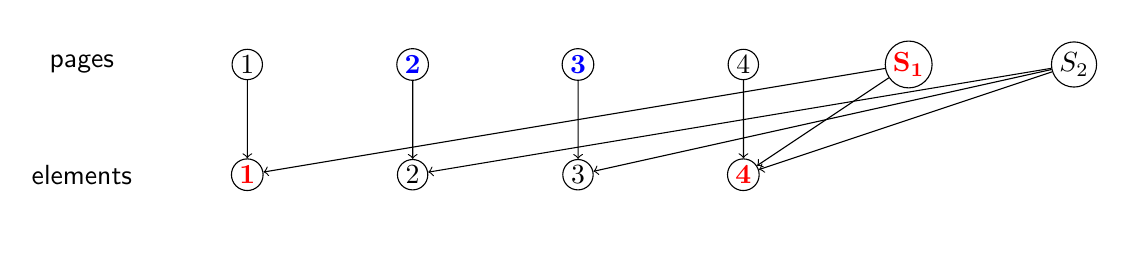
\begin{tikzpicture}[scale=1.4, every node/.style={draw, circle, inner sep=1pt}]
			% first bipartite graph
			\node (p2) at (5.5,-0.5) {$\bf \textcolor{blue}{2}$};
			\node (p1) at (4,-0.5) {$\textcolor{black}{1}$};
			\node (p3) at (7,-0.5) {$\bf \textcolor{blue}{3}$};
			\node (a1) at (4,-1.5) {$\bf \textcolor{red}{1}$};
			
			\node (a2) at (5.5,-1.5) {$\textcolor{black}{2}$};
			\node (a3) at (7,-1.5) {$\textcolor{black}{3}$};
			\node (a4) at (8.5,-1.5) {$\bf \textcolor{red}{4}$};
			\node (p4) at (8.5,-0.5) {$4$};
			
				\node (S1) at (10,-0.5) {$\bf \textcolor{red}{S_1}$};
				
					\node (S2) at (11.5,-0.5) {$S_2$};
	\draw[->] (S1) -- (a1);
	
		\draw[->] (S2) -- (a3);
			\draw[->] (S2) -- (a4);
				\draw[->] (S2) -- (a2);
				
		\draw[->] (S1) -- (a4);			
			\draw[->] (p1) -- (a1);
				\draw[->] (p2) -- (a2);
					\draw[->] (p3) -- (a3);
						\draw[->] (p4) -- (a4);
			%		\draw (p3) -- (a2);
			%	\draw[line width=2pt, color=red] (p3) -- (a3);
			
%			\draw[->] (p3) -- (a3);
%			\draw[->] (p2) -- (a1);
%			\draw[->] (p1) -- (a2);
%			\draw[->] (p2) -- (a3);
%			
%			\draw[->] (p4) -- (a2);
%			\draw[->] (p4) -- (a3);
%			\draw[->] (p4) -- (a4);
			
			
			\node[draw=none] at (2.5, -0.5) {$\textsf{pages}$};
			
			\node[draw=none] at (2.5, -1.5) {$\textsf{elements}$};
			
		\end{tikzpicture}
		%\vspace{-1.5cm} 
		\caption{\label{fig:Y} An illustration of the construction for $X = \{1,\ldots,4\}$ and $\cS = \{S_1,S_2\}$. The considered moment in time takes place after a request for element-pages $1,4$; to serve these requests, the set-page $S_1$ (in red) is evicted from cache (taken to the cover). Observe that $\{2,3,S_1\}$, the pages outside of the cache, form a feasible cover of the elements $\{1,\ldots,4\}$.}
	\end{figure}
 
%\begin{lemma}
%	\label{lem:Set Cover}
%	For any $\rho \geq 1$, if there is a $\rho$-competitive algorithm for \textnormal{supermodular paging} then there is a $\rho$-competitive algorithm for \textnormal{online set cover} of the same running time up to a polynomial factor.  
%\end{lemma}
Observe that in our reduction $|\cP| = m+n$ and that $f(\cP) = n$. Thus, by \Cref{lem:Set Cover} and the results of \cite{alon2003online,korman2004use}, we have the statement of \Cref{thm:hardness}. %(for $f(\cP) = \Omega(n)$).




\subsubsection*{Proof of \Cref{thm:LB}}

By the results of \cite{korman2004use}, there are constants $a,b>0$ such that there are online set cover instances with $n$ elements, $m = n^a$ sets such that the minimum number of sets required to form a feasible cover at the end of the algorithm is $K = n^b$ and no randomized online algorithm is $\Omega(\log^2\left(n\right))$-competitive on these instances unless $\textnormal{NP}\subseteq \textnormal{BPP}$. Moreover, note that the cardinality of the maximum minimally infeasible set (see \Cref{def:Mininfeasible}) is at least $K = n^b$ and at most $n$; thus, $\ell$ is polynomial in $n$ i.e., there is a constant $c>0$ such that $\ell = n^c$. Therefore, the lower bound on the running time obtained by \Cref{lem:Set Cover} combined with \cite{korman2004use} is $\Omega(\log^2\left(\ell\right)) = \Omega(\log^2\left(n\right))$. \qed


\subsection{Hardness of Restricted Non-linear Paging instances}
\label{sec:hardRestricted}

We now show that even for very restricted cases of the problem, the competitive ratio is effectively unbounded (if the competitive ratio is not stated as a function of $\ell$ or $n$). 

\begin{theorem}
\label{thm:HardnessRestricted}
For every $\rho \geq 1$, there is no randomized or deterministic $\rho$-competitive algorithm for \textnormal{non-linear paging} even if $k = 0$ and the range of $f$ is $\{0,1\}$.
\end{theorem}

\begin{proof}
We give a reduction from the classic paging problem. Let $I$ be a paging instance with a set $\cP$ of $n+1$ pages, cache capacity $n$, and requests $p_t$ for every point of time $t \in T$. We define a non-linear paging instance $R$ as follows. The set of pages and requests are the same in $I$ and $R$. Define a feasibility function $f:\cP \rightarrow \{0,1\}$ such that for every $S \subseteq \cP$ it holds that $f(S) = 0$ if $|S| \leq n$ and $f(S) = 1$ otherwise. Finally, define $k = 0$ as the cache size constraint of $R$. Clearly, a subset of pages $S \in \cP$ is feasible for $I$ if and only if it is feasible for $R$. Thus, by the well-known hardness results for deterministic paging, we cannot obtain better than $n$-competitive \cite{sleator1985amortized} (recall that the instance has $n+1$ pages and the cache capacity is $n$); if randomization is allowed, we cannot obtain better than $O(\log n)$-competitive \cite{fiat1991competitive}. As $n$ can be arbitrarily large, we prove the theorem.  
    %Fix some integer $\rho \geq 1$
\end{proof}